% Author: Alfredo Sánchez Alberca (asalber@ceu.es}
% !TEX program = xelatex
\documentclass[aspectratio=149,10pt,t]{beamer}
%-------------------------------------------------------------------------------
% GENERAL PACKAGES
%-------------------------------------------------------------------------------
% Language
\usepackage{polyglossia}
\setdefaultlanguage{spanish}
% Maths
\usepackage{amsmath} % Math symbols and environments
\usepackage{amsfonts}
\usepackage{amssymb}
% Tables
\usepackage{array}
\usepackage{multirow}
% Graphics
\usepackage{graphicx}
\usepackage{tikz}
\usetikzlibrary{positioning}


% Colors
\definecolor{blueceu}{RGB}{0,164,227}
\definecolor{greenceu}{RGB}{194,205,24}
\definecolor{redceu}{RGB}{238,50,36}
\definecolor{purpleceu}{RGB}{169,78,145}
\definecolor{greyceu}{RGB}{117,117,97}
\definecolor{darkgrey}{RGB}{40,40,50}
\definecolor{softblueceu}{RGB}{193,225,246}
\setbeamercolor{structure}{fg=blueceu}
\setbeamercolor{normal text}{fg=darkgrey}
\hypersetup{colorlinks, urlcolor=purpleceu}

%-------------------------------------------------------------------------------
% FONTS
%-------------------------------------------------------------------------------
\usepackage{fontspec}
\setmainfont[Ligatures=TeX]{TeX Gyre Pagella}
\usepackage{unicode-math}
\setmathfont[math-style=ISO,bold-style=ISO,vargreek-shape=TeX]{TeX Gyre Pagella Math}
% Creative common icons
\usepackage[scale=1.5]{ccicons}

%-------------------------------------------------------------------------------
% CONFIGURATION
%-------------------------------------------------------------------------------
\setbeamersize{text margin left=.5cm, text margin right=.5cm} % Defines margin sizes
\beamertemplatenavigationsymbolsempty % Hide navitation bar
\usefonttheme[onlymath]{serif} % Math text in serif
\setbeamertemplate{blocks}[rounded] % Blocks with rounded corners
%\setbeamercolor{block title}{bg=RoyalBlue!10} % Color of block title
%\setbeamercolor{block body}{bg=RoyalBlue!10} % Color of block body


%-------------------------------------------------------------------------------
% DOCUMENT
%-------------------------------------------------------------------------------
\begin{document}
%---------------------------------------------------------------------SLIDE----
\begin{frame}[c]
\vspace{1.5cm}

\begin{center}
\structure{\LARGE {\textbf{Ejercicios de Estadística}}}
\bigskip

\large
\begin{tabular}{rl}
Temas: & \structure{Probabilidad: Tests diagnósticos}\\
Titulaciones: & \structure{Todas}
\end{tabular}

\bigskip
Alfredo Sánchez Alberca\\
\url{asalber@ceu.es}\\
\url{http://aprendeconalf.es}\\


\includegraphics[scale=0.2]{../img/logo_uspceu}

\bigskip
{\color{darkgrey}\ccbyncsaeu}
\end{center}
\end{frame}


%----------------------------------------------------------------------SLIDE----
\begin{frame}[c]
	\large
	Para detectar una enfermedad con una prevalencia del 10\% se dispone de un test diagnóstico con una sensibilidad del 95\% y una especificidad del 85\%.
	Se pide:
	\begin{enumerate}
	  \item Calcular los valores predictivos positivo y negativo del test e interpretarlos.
	  ¿Se trata de un test más útil para detectar la enfermedad o para descartarla?
	  \item ¿Cuál debería la especificidad del test para que el valor predictivo positivo fuera del 80\%?
	\end{enumerate}
\end{frame}


%----------------------------------------------------------------------SLIDE----
\begin{frame}
	\begin{columns}
		\begin{column}[T]{0.6\textwidth}
			Para detectar una enfermedad con una prevalencia del 10\% se dispone de un test diagnóstico con una sensibilidad del 95\% y una especificidad del 85\%.
		\end{column}
		\begin{column}[T]{0.4\textwidth}
			\structure{Datos}\\
			$E \equiv$ Tener la enfermedad\\
			$+ \equiv$ Resultado del test positivo\\
			$- \equiv$ Resultado del test negativo\\
			Prevalencia: $P(E):0.1$\\
			Sensibilidad: $P(+|E)=0.95$\\
			Especificidad: $P(-|\overline E)=0.85$
		\end{column}
	\end{columns}
\end{frame}


%----------------------------------------------------------------------SLIDE----
\begin{frame}
	\begin{columns}
		\begin{column}[T]{0.5\textwidth}
			\begin{enumerate}
			  \item Calcular los valores predictivos positivo y negativo del test e interpretarlos.
			  ¿Se trata de un test más útil para detectar la enfermedad o para descartarla?
			\end{enumerate}
		\end{column}
		\begin{column}[T]{0.5\textwidth}
			\structure{Datos}
			\medskip

			\resizebox{\textwidth}{!}{
			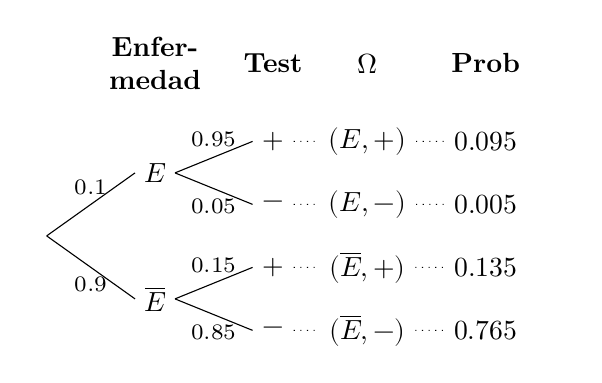
\begin{tikzpicture}[
			grow'=right,
			level 1/.style ={level distance=1.5cm, sibling distance=1.6cm, parent anchor=east, child anchor=west},
			level 2/.style ={level distance=1.5cm, sibling distance=0.8cm},
			level 3/.style ={level distance=1.2cm, sibling distance=0.8cm, dotted},
			level 4/.style ={level distance=1.5cm, sibling distance=0.8cm, dotted},
			prob/.style={font=\footnotesize,above}
			]

			\node (root) {}
				child {node {$E$}
					child {node {$+$}
						child {node{$(E,+)$}
							child {node{$0.095$}}
						}
						edge from parent node[prob] {$0.95$}
					}
					child {node {$-$}
						child {node{$(E,-)$}
							child {node{$0.005$}}
						}
						edge from parent node[prob,below] {$0.05$}
					}
					edge from parent node[prob] {$0.1$}
				}
				child {node {$\overline E$}
			   		child {node {$+$}
						child {node{$(\overline E,+)$}
							child {node{$0.135$}}
						}
						edge from parent node[prob] {$0.15$}
					}
					child {node {$-$}
						child {node{$(\overline E,-)$}
							child {node{$0.765$}}
						}
						edge from parent node[prob,below] {$0.85$}
					}
					edge from parent node[prob,below] {$0.9$}
				};

			\begin{scope}[every node/.style={text width=2cm, align=center, anchor=center, font=\bfseries,}]
			\node[above= 0.5cm of root-1-1-1-1] (labels-level) {Prob};
			\node[at =(labels-level-|root-1-1-1)] {$\Omega$};
			\node[at =(labels-level-|root-1-1)] {Test};
			\node[at =(labels-level-|root-1)] {Enfermedad};
			\end{scope}
		\end{tikzpicture}}
		\end{column}
	\end{columns}
\end{frame}


%----------------------------------------------------------------------SLIDE----
\begin{frame}
	\begin{columns}
		\begin{column}[T]{0.5\textwidth}
			\begin{enumerate}
			  \item[2.] ¿Cuál debería la especificidad del test para que el valor predictivo positivo fuera del 80\%?
			\end{enumerate}
		\end{column}
		\begin{column}[T]{0.5\textwidth}
			\structure{Datos}
			\medskip

			\resizebox{\textwidth}{!}{
			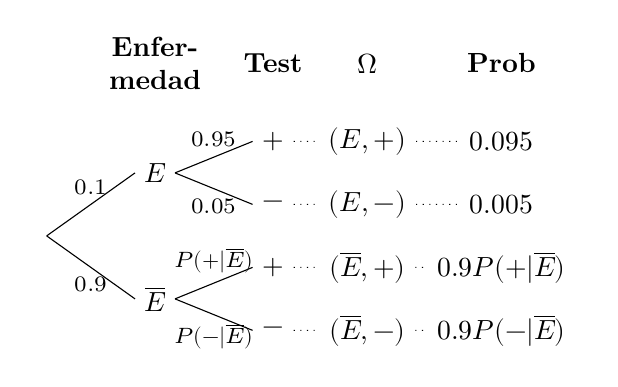
\begin{tikzpicture}[
			grow'=right,
			level 1/.style ={level distance=1.5cm, sibling distance=1.6cm, parent anchor=east, child anchor=west},
			level 2/.style ={level distance=1.5cm, sibling distance=0.8cm},
			level 3/.style ={level distance=1.2cm, sibling distance=0.8cm, dotted},
			level 4/.style ={level distance=1.7cm, sibling distance=0.8cm, dotted},
			prob/.style={font=\footnotesize,above}
			]

			\node (root) {}
				child {node {$E$}
					child {node {$+$}
						child {node{$(E,+)$}
							child {node{$0.095$}}
						}
						edge from parent node[prob] {$0.95$}
					}
					child {node {$-$}
						child {node{$(E,-)$}
							child {node{$0.005$}}
						}
						edge from parent node[prob,below] {$0.05$}
					}
					edge from parent node[prob] {$0.1$}
				}
				child {node {$\overline E$}
			   		child {node {$+$}
						child {node{$(\overline E,+)$}
							child {node{$0.9P(+|\overline E)$}}
						}
						edge from parent node[prob] {$P(+|\overline E)$}
					}
					child {node {$-$}
						child {node{$(\overline E,-)$}
							child {node{$0.9 P(-|\overline E)$}}
						}
						edge from parent node[prob,below] {$P(-|\overline E) $}
					}
					edge from parent node[prob,below] {$0.9$}
				};

			\begin{scope}[every node/.style={text width=2cm, align=center, anchor=center, font=\bfseries,}]
			\node[above= 0.5cm of root-1-1-1-1] (labels-level) {Prob};
			\node[at =(labels-level-|root-1-1-1)] {$\Omega$};
			\node[at =(labels-level-|root-1-1)] {Test};
			\node[at =(labels-level-|root-1)] {Enfermedad};
			\end{scope}
		\end{tikzpicture}}
		\end{column}
	\end{columns}
\end{frame}

\end{document}
